\chapter{Transformers}


\begin{figure}[h!]
  \centering
  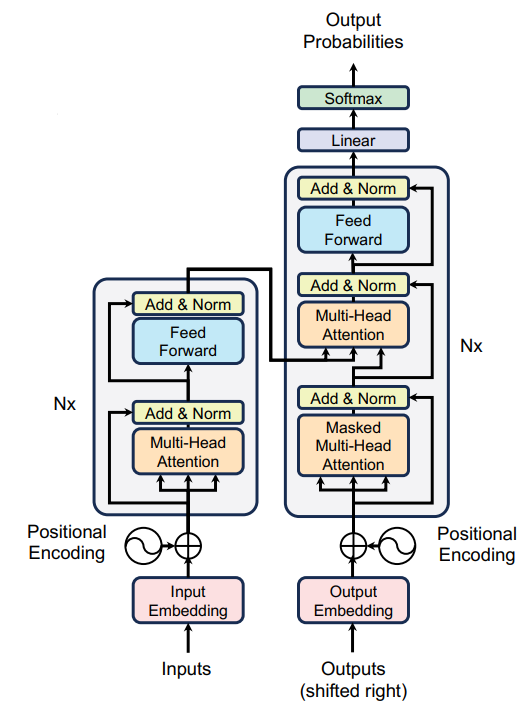
\includegraphics[width=0.3\linewidth]{content/Parts/images/2026-09-30-11-47-27.png}
\end{figure}

Transformers architecture are not longer based on RNN. We shot the model the entire sequence
wery puerfull, but is expencive.

\section{Simplified architecture}

\begin{center}
  \begin{minipage}{0.65\linewidth}

    We need yellow imputes and the model give us the green outputs.

  \end{minipage}%
  \hfill
  \begin{minipage}{0.3\linewidth}
    \centering
    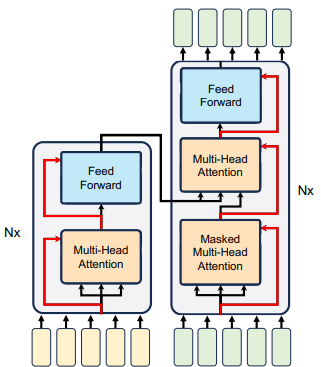
\includegraphics[width=0.3\linewidth]{content/Parts/images/2026-09-30-11-49-14.png}
  \end{minipage}
\end{center}

We have two types of inputs:
\begin{itemize}
  \item FF - Feed forward
\end{itemize}


\section{Generation the first token}

The input sequence  pass to encoder model and the output of the encoder producers a vector for each
token provided in input. 10 input 10 output, is a property of the attenction layer, this means no compression
in a single vector and no loss of information if it is a good encoder.

The decoder takes the output of the encoder and we need to speciify the first token, we give the
special vector. The model will look it and decide then it prdoduce output 1 input 1 output (BOS).
The output is always a probabiilty function in our vocaboly.
That word become the second word on the decoder input.
The encoder knows the intire previous sequence, at the end we produce a end of sequence token (EOS).

\begin{tcolorbox}
  \textbf{Note}: The decoder will output a prediction for each input token. At inference
  time, we are interested the latest generated token. At training time,
  the loss is computed on all tokens generated at that step!
\end{tcolorbox}

Cosality masking, 2 input 2 output, but the first token LLM should not see on the GUI, it already printed.



\section{Tokenization}

We need a way to split a sentence into units. This process is called tokenization, and splits the sequence into tokens

Transformers need to process natural language, in the form of sentences, braking into small units.


\subsubsection{Character-level}

\begin{figure}[h!]
  \centering
  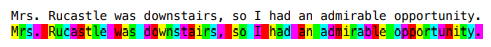
\includegraphics[width=0.3\linewidth]{content/Parts/images/2026-09-30-12-11-59.png}
\end{figure}

Braking up the sentence into characters. Each character is a token.

\begin{flushleft}
  \begin{minipage}[t]{0.45\linewidth}
    \raggedright
    Pros:

    \begin{itemize}
      \item Simple solutions
      \item No out-of-vocabulary problem
      \item Robust to misspellings and variations
    \end{itemize}
  \end{minipage}%
  \hfill
  \begin{minipage}[t]{0.45\linewidth}
    \raggedright

    Cons:
    \begin{itemize}
      \item Long sequences - transformers, attention mechanisms, are $O(N^2)$ in the sequence length
      \item Slower/more complex training
      \item Semantic information is harder to capture
      \item Inefficient for common words
    \end{itemize}

  \end{minipage}
\end{flushleft}



\subsubsection{Word-level}

Breaks text into individual words. Each word is treated as as token

\begin{figure}[h!]
  \centering
  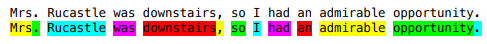
\includegraphics[width=0.3\linewidth]{content/Parts/images/2026-09-30-12-18-02.png}
\end{figure}

\begin{flushleft}
  \begin{minipage}[t]{0.45\linewidth}
    \raggedright
    Pros:

    \begin{itemize}
      \item Captures semantic meaning directly
      \item Shorter sequences compared to character-level
      \item More intuitive/easier to understand
    \end{itemize}
  \end{minipage}%
  \hfill
  \begin{minipage}[t]{0.45\linewidth}
    \raggedright

    Cons:
    \begin{itemize}
      \item Out-of-vocabulary (OOV) issues for rare or new words
      \item Does not leverage some information shared among words (e.g. prefixes/suffixes)
      \item Larger vocabulary needed, leading to memory inefficiency
      \item Vectors for rarer words are trained “less”
    \end{itemize}

  \end{minipage}
\end{flushleft}

\subsubsection{Subword-level}

Breaks text into subword units (e.g., prefixes, suffixes). fastText uses n-grams contained in each word.
A more commonly used method is Byte-Pair Encoding (BPE)

\begin{figure}[h!]
  \centering
  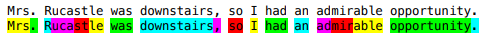
\includegraphics[width=0.3\linewidth]{content/Parts/images/2026-09-30-12-19-53.png}
\end{figure}


\begin{flushleft}
  \begin{minipage}[t]{0.45\linewidth}
    \raggedright
    Pros:

    \begin{itemize}
      \item Balances between character-level and word-level
      \item Handles out-of-vocabulary words effectively
      \item Compact vocabulary with better generalization
      \item Efficient for both frequent and rare words
    \end{itemize}
  \end{minipage}%
  \hfill
  \begin{minipage}[t]{0.45\linewidth}
    \raggedright

    Cons:
    \begin{itemize}
      \item Common words are represented by fewer subwords w.r.t. rarer words
      \item Requires defining a subword definition policy
      \item The subword definition policy may introduce some computational overhead
    \end{itemize}

  \end{minipage}
\end{flushleft}


In practice, subword-level is the most commonly adopted tokenization method.
A simple, yet commonly adopted technique is BPE - Byte-Pair Encoding.

\section{Byte-Pair Encoding - desiderata}

Data driven approach is used to chose "best" tokens. To do so, we need a colection of text called
\textbf{corpus}.

\begin{itemize}
  \item Common words to be encoded into a single token
  \item Rare words to be encoded into multiple tokens
\end{itemize}

Also we difeine the desired maximum number of tokens


\begin{enumerate}
  \item The corpus is initially encoded with 1 carachers byte  = 1 token so we address all possible
        sentences.
  \item We count the frequency of each pair of subsequent tokens is countd in the copus
  \item The mosr frequent pair of tokens ($F_1, F_2$) is assiged a new token $T$
  \item All occurrences of the pair ($F_1, F_2$) in the corpus are replaced with $T$
  \item The process 2-4 is repeated until the desired number of tokens is reached
\end{enumerate}

\paragraph{BPE example}: The corpus we we would use as example is "would a woodchuck chuck wood"

\begin{itemize}
  \item Corpus: "would a woodchuck chuck wood"
  \item Initial encoding: w | o | u | l | d |  | a |  | w | o | o | d | c | h | u | c | k |   | c | h | u | c | k |  | w | o | o | d
  \item Count frequency of pairs: (w, o): 3, (o, o): 2 \dots
  \item Assign a new token to the most frequent pair: (w, o) → wo
\end{itemize}

\begin{figure}[h!]
  \centering
  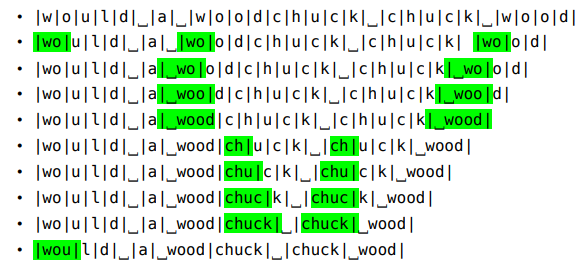
\includegraphics[width=0.3\linewidth]{content/Parts/images/2026-09-30-12-37-40.png}
\end{figure}

\subsection{BPE results}

\begin{figure}[h!]
  \centering
  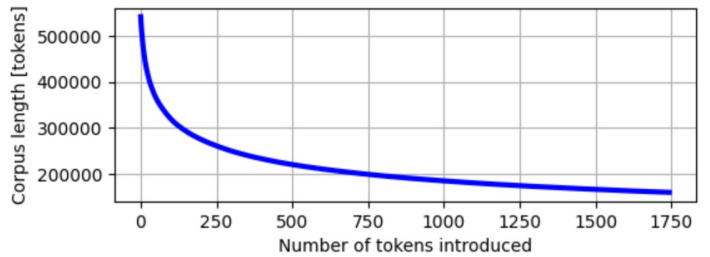
\includegraphics[width=0.3\linewidth]{content/Parts/images/2026-09-30-12-39-33.png}
\end{figure}

The number of tokens used to represent the corpus decreases as we
increase the number of tokens used. There is a reasonable small number of tokens that can be used
to represent a large corpus.

Typically, 10's to 100's of thousands of tokens are used

\section{Some extra tokens}

We introduce some special tokens to indicate that special positions
within a sequence. For instance, we can use tokens for beginning/end of sequence during training.

\begin{itemize}
  \item BOS - Beginning of Sequence
  \item EOS - End of Sequence
  \item CLS - Classification token for task-specific use
  \item SEP - Separator token within the same input. E.g. Separate Question from Answer in Question Answering tasks
\end{itemize}


\section{Positional encoding}

Every time we have a token is associated to a vector learned during the training, start with random vectors, and
adjust them via gradient descent.

The \textbf{same token} is mapped to the \textbf{same vector} regardless of its position in the sequence.
This is not ideal. Additionlly the \textbf{Attentiona and Feed Forward does not understand the order} of the elements.

We have to figure it out a way to inject the position before passing it to the transformer.
This is called \textbf{positional encoding}.

\begin{figure}[h!]
  \centering
  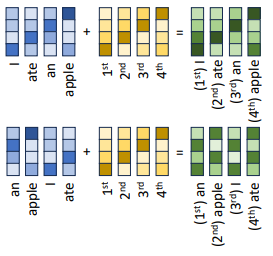
\includegraphics[width=0.3\linewidth]{content/Parts/images/2026-09-30-12-50-39.png}
\end{figure}

\section{Sinusoidal Positional encoding}

In the paper "Attention is all you need" Google engineers proposed a sinusoidal positional encoding.


In the AIAYN paper, the PE
vectors are defined as:

\begin{equation*}
  \begin{aligned}
    PE_{(pos, 2i)} = sin( \frac{pos}{10000^{2i/d_{model}}}) \\
    PE_{(pos, 2i+1)} = cos( \frac{pos}{10000^{2i/d_{model}}})
  \end{aligned}
\end{equation*}

where $pos$ is the position of the token we have some dependencies. 10000 is a magic number
often used in smaller transformer architecture.
$i$ the position of the dimension we are filling.
$d_{model}$ is the dimension of the model, how big are the vectors.


\begin{center}
  \begin{minipage}{0.47\linewidth}
    \centering
    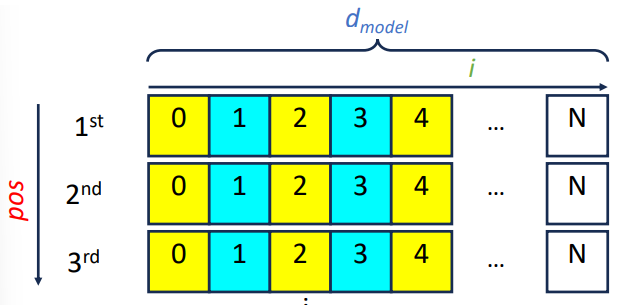
\includegraphics[width=0.9\linewidth]{content/Parts/images/2026-10-05-08-38-53.png}
  \end{minipage}
  \hfill
  \begin{minipage}{0.47\linewidth}
    \centering
    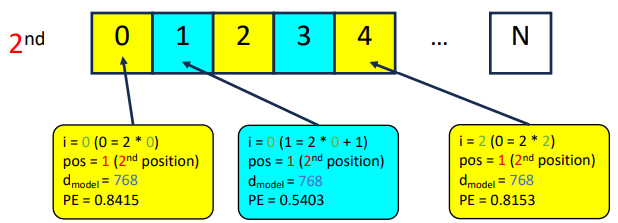
\includegraphics[width=0.9\linewidth]{content/Parts/images/2026-10-05-08-39-30.png}
  \end{minipage}
\end{center}

\begin{tcolorbox}
  \textbf{Error:} in the blue box the formula should be $i = 1$
\end{tcolorbox}

\begin{center}
  \begin{minipage}{0.65\linewidth}

  \end{minipage}%
  \hfill
  \begin{minipage}{0.3\linewidth}
    \centering
    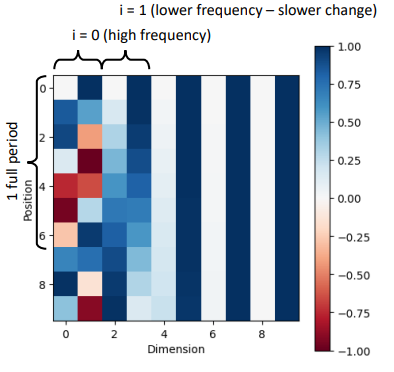
\includegraphics[width=0.3\linewidth]{content/Parts/images/2026-10-05-08-51-52.png}
  \end{minipage}
\end{center}

\begin{figure}[h!]
  \centering
  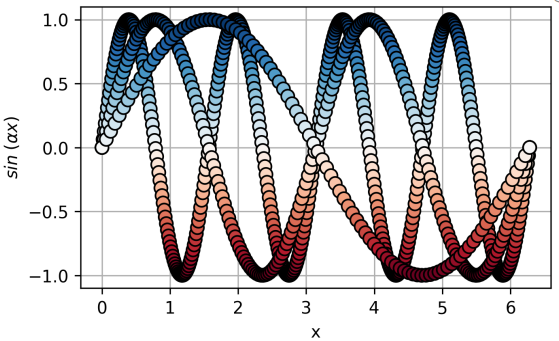
\includegraphics[width=0.3\linewidth]{content/Parts/images/2026-10-05-08-52-24.png}
\end{figure}

\subsection{Positional encoding uniqueness}
The vector for each position is
unique… At least for the first  $~60K$ positions ($2\pi \cdot 10000$).
then they start repeating (for
longer sequences, we can just
change the $10K$ constant!)

\section{Positional encoding preserves similarity}
If position 1 is close to position 2
(e.g., the third vs the fourth words
in a sentence) we want positional
vectors to also be close!
We can easily verify that using
trigonometric functions ensures
that this is the case

Example for max position = 1,000
and dmodel = 768


Cosine similarity of each pair of the
previous positional vectors

Maximum similarity along the
diagonal (of course)

\begin{figure}[h!]
  \centering
  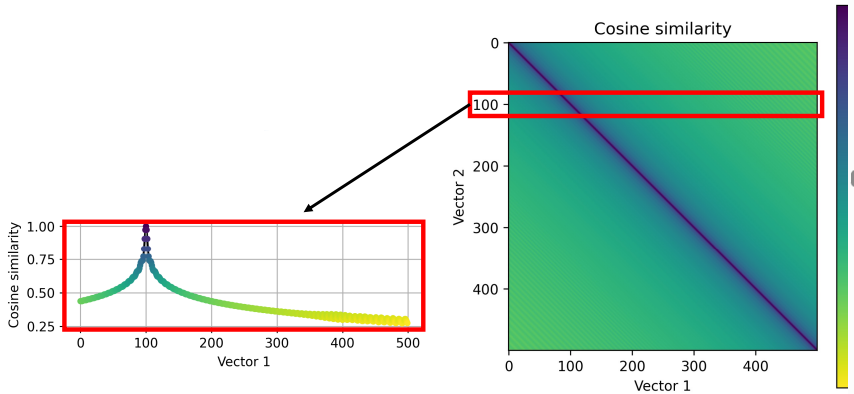
\includegraphics[width=0.3\linewidth]{content/Parts/images/2026-10-05-09-01-21.png}
\end{figure}


\subsection{Learned positional embeddings}
After the first transformer paper, other people proposed other solutions for positional encoding.
Some model e.g. GPT family uses posisitona embeddings.
This approach was also considered in AIAYN,
but discarded as it did not produce better
results

\section{Attention}

\begin{figure}[h!]
  \centering
  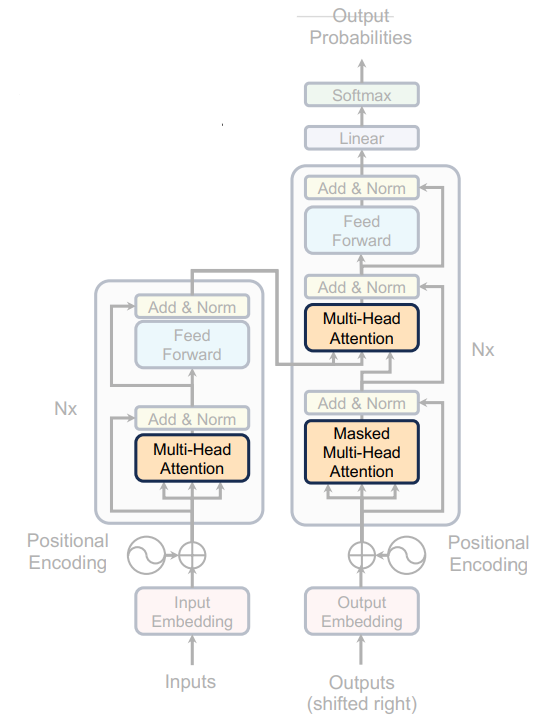
\includegraphics[width=0.3\linewidth]{content/Parts/images/2026-10-05-09-08-00.png}
\end{figure}

\begin{center}
  \begin{minipage}{0.65\linewidth}
    “How much” of each other vector is added is
    defined by the attention paid to them. Ideally, useful tokens will be weighted a lot.
    Unuseful tokens will be weighted less

    The transformer learns to choose these
    weights based on the input sequence

    Weight sum of the input  = Attention


    The attention module requires:  An input (to be contextualized) and A way to define the attention weights
    The i-th output is defined as
    \begin{equation*}

      out_i = \sum_{j} Attn\_weight{i,j} \cdot f(in_j)
    \end{equation*}

  \end{minipage}%
  \hfill
  \begin{minipage}{0.3\linewidth}
    \centering
    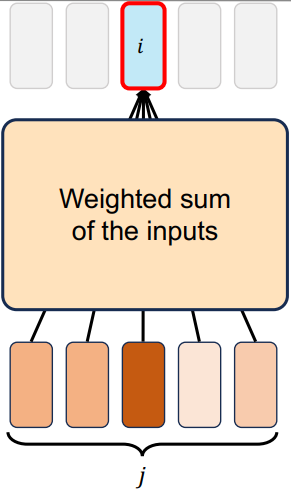
\includegraphics[width=0.3\linewidth]{content/Parts/images/2026-10-05-09-12-38.png}
  \end{minipage}
\end{center}

\subsection{Classic dictionary lookup}
A small digression




\subsection{Dot-product attention - Weighted lookup}


\subsection{Attention as Keys/Values/Queries}
We expect to have multiple queries with three seprate "inputs":

\begin{itemize}
  \item Queries: the value to be looked up, we want 1 output fro each query
  \item Keys: the values to be matched against the queries
  \item Values: the values associated to each key
\end{itemize}

This is why the 3-inputs block in the
transformers' architecture

\subsection{the 3-inputs block in the transformers' architecture}

How to to compute the attention weights? Since the dot function produce unbounded values,
we need to normalize them. We can use the softmax.


\subsection{Packing everything into matrices}

\begin{center}
  \begin{minipage}{0.65\linewidth}

    We discussed the situation having a single
    query. Of course, we can have multiple queries,
    each treated in the same way

  \end{minipage}%
  \hfill
  \begin{minipage}{0.3\linewidth}
    \centering
    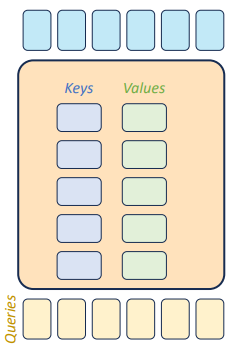
\includegraphics[width=0.3\linewidth]{content/Parts/images/2026-10-05-09-25-35.png}
  \end{minipage}
\end{center}





For convenience, we can summarize the set of all queries, keys and values
as three matrices, Q, K, V.

\begin{itemize}
  \item Q: contains N queries, each being a $d_k$-dimensional vector
  \item K: contains M entries, each being a $d_k$-dimensional vector
  \item V: contains M entries (one value for each key), each being a $d_v$-dimensional vector output
\end{itemize}

\begin{figure}[h!]
  \centering
  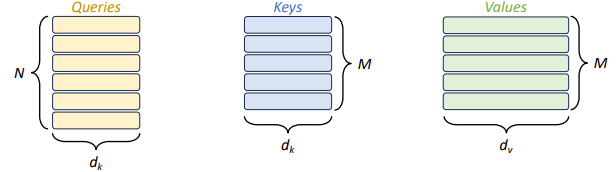
\includegraphics[width=0.3\linewidth]{content/Parts/images/2026-10-05-09-24-00.png}
\end{figure}

\section{Scaled Dot-product attention}

In the original transformers, the final attention is defined as:

\begin{equation*}
  Attention(Q, K, V) = softmax(\frac{QK^T}{\sqrt{d_k}})V
\end{equation*}

\begin{itemize}
  \item $QK^T$: efficiently computes the dot product between each query and each key.
        This produces an $N \times M$ matrix
\end{itemize}


\subsection{Attention example}



\subsection{Types of attention}
Attention is used in three situations
in the classic transformer
architecture.

The first one is called the encoder self-attention, Decoder self-attention, and the third one is called encoder-decoder cross attention.



\subsubsection{Encoder self-attention}





\subsubsection{Decoder (masked) self-attention}

This is the block used by the decoder. Used on the output tockens.

It looks only what has been generated so far, and not the future tokens.



\subsubsection{Encoder-decoder cross-attention}

Type of attention where part of the input comes from the encoder and part comes from the decoder.

The decoder produce the output and the cross attention, keys and values come from the encoder.


\section{Multi-head attention}




\begin{center}
  \begin{minipage}{0.65\linewidth}
    Each of the block before are multi-head attention, with its own $W^Q$, $W^K$, $W^V$ .
    Since the attention may need to focus on different aspects in different
    contexts, we generally adopt multiple attention heads in parallel.

    So far we discussed the attention mechanism with a single head.


    The final attention output is the concatenation of the various heads'
    outputs. Passed through a linear layer to go back to the desired vector size.

  \end{minipage}%
  \hfill
  \begin{minipage}{0.3\linewidth}
    \centering
    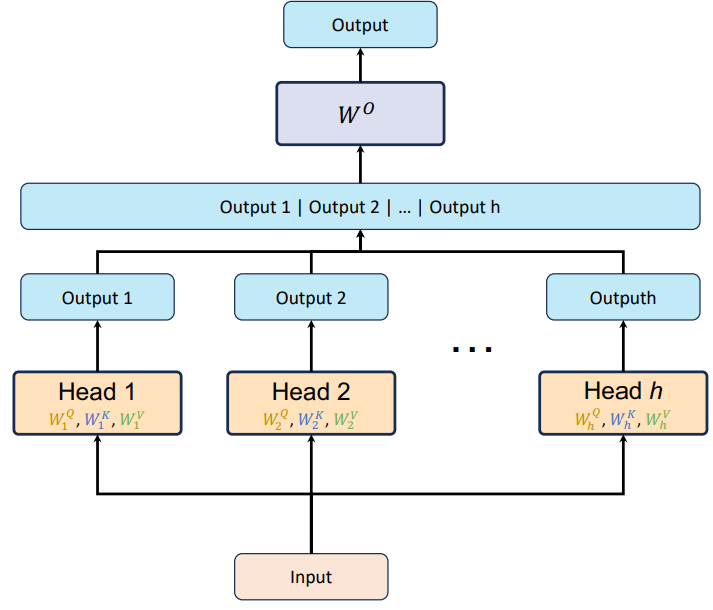
\includegraphics[width=0.3\linewidth]{content/Parts/images/2026-10-05-10-26-21.png}
  \end{minipage}
\end{center}


\section{Some additional details}

\subsection{Residual connections}


\begin{center}
  \begin{minipage}{0.65\linewidth}
    Residual connections are a technique used to improve
    gradient flow in backpropagation.

    The gradient “skips” part of the network when being
    backpropagated. Indeed, these are sometimes called skip connections.

    Is a shortcut to make it easyer non-zero signal to flow through the network.

    The output is the sum of the input plus the input $out = f(x) + x$



  \end{minipage}%
  \hfill
  \begin{minipage}{0.3\linewidth}
    \centering
    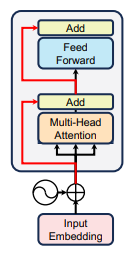
\includegraphics[width=0.3\linewidth]{content/Parts/images/2026-10-05-10-28-14.png}
  \end{minipage}
\end{center}

\subsection{Layer Normalization}


\begin{center}
  \begin{minipage}{0.65\linewidth}
    Add is the residual part, and Nord is the normalization layer. Such as single token vector, we
    normalize that across all deminsion a specific variance and a speicifi

    This makes the training faster and more stable.

    \begin{equation*}
      y = \frac{x - E[x]}{\sqrt{Var[x] + \epsilon}} \cdot \gamma + \beta
    \end{equation*}

    Where $\gamma$ and $\beta$ are learnable parameters, and $\epsilon$ is a small constant to avoid division by zero.

  \end{minipage}%
  \hfill
  \begin{minipage}{0.3\linewidth}
    \centering
    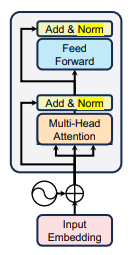
\includegraphics[width=0.3\linewidth]{content/Parts/images/2026-10-05-10-32-02.png}
  \end{minipage}
\end{center}


\subsection{Actual connections}


\begin{center}
  \begin{minipage}{0.65\linewidth}

    The encoder and decoder are stacked in this way.
    The output of the final encoder block becomes the input of the cross attentions of all the decoder.
    The cross attention only takes the output of the last encoder block.

    This means no match between encoder and decoder block, e.g. encoder can >> decoder, or vice versa.
    Normally are the same number of blocks, but not necessary.

  \end{minipage}%
  \hfill
  \begin{minipage}{0.3\linewidth}
    \centering
    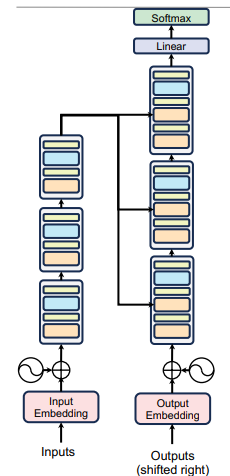
\includegraphics[width=0.3\linewidth]{content/Parts/images/2026-10-05-10-39-11.png}
  \end{minipage}
\end{center}


\subsection{Relative positional embeddings}


\begin{center}
  \begin{minipage}{0.65\linewidth}

    AIAYN uses sinusoidal absolute positional encoding, other, like GPT family, uses learned
    absolute positional embeddings.

    This means there are different type of positional encoding.

    Relative positional embeddings: one position of a sentence maps to one vector, but some
    people proposed to use relative positional changes for each words and the words
    near it.

    Positional information no longer introduced in the input
    vectors, but at “attention time”. We build vecrtor with a fixed size window.

    Not applicable at the beginning but after compute the key score, when we have the
    relation.


    Nowadays we use a mix of all the techniques.


  \end{minipage}%
  \hfill
  \begin{minipage}{0.3\linewidth}
    \centering
    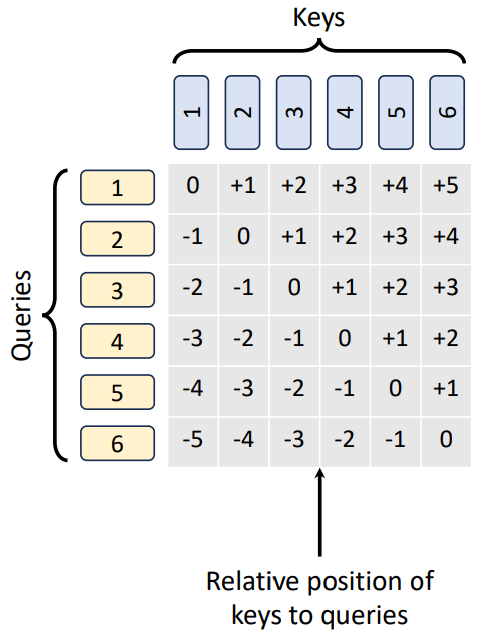
\includegraphics[width=0.3\linewidth]{content/Parts/images/2026-10-05-10-41-26.png}
  \end{minipage}
\end{center}


\subsection{Advantages of transformers}


\begin{itemize}
  \item \textbf{Parallelization}: Transformers can process all tokens simultaneously, no dep on previous states.
        Remember, we use teacher forcing to ``know the future'' -  no need to wait
        for autoregressive generation
  \item \textbf{Long-range relationships}: With attention, Transformers can see the entire sequence at all times, and
        choose what to pay attention to. The model does not need to remember because it receave all the input context and use the
        attention mechanism to focus on the relevant parts. This implies that each token looks at all tokens, this is N2 and represents
        one of the current limitations of Transformers.
  \item \textbf{Better memory}: Since there is no sequential processing, forgetting issues generally do not occur
\end{itemize}




\section{Encoder-decoder architecture}


\begin{center}
  \begin{minipage}{0.65\linewidth}

    The famous example is the T5 - Text-to-Text Transfer Transformer.

    This ia a vanilla endoder-decoder transformer. \textbf{Single framework}, same weights, for
    multiple tasks.

    Summarization, translation.

    How does it works?

    We have one sentence and we add a prefix to the input, e.g. "summarize: " or "translate" to predend or
    append to the text, learned to the model.

    Task prefixes to condition the decoder's output, instead of using different architectures.

  \end{minipage}%
  \hfill
  \begin{minipage}{0.3\linewidth}
    \centering
    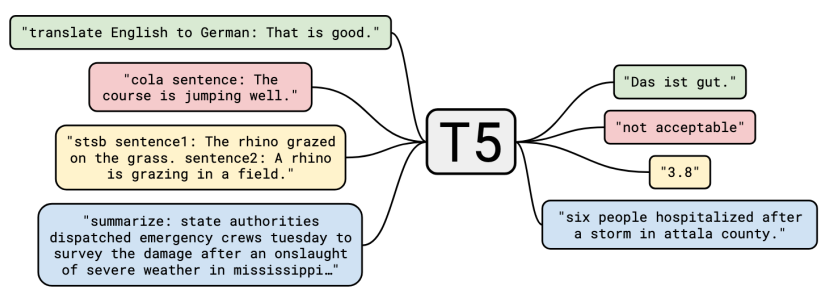
\includegraphics[width=0.3\linewidth]{content/Parts/images/2026-10-05-10-55-57.png}
  \end{minipage}
\end{center}

\subsection{Single model, multiple tasks!}


\begin{figure}[h!]
  \centering
  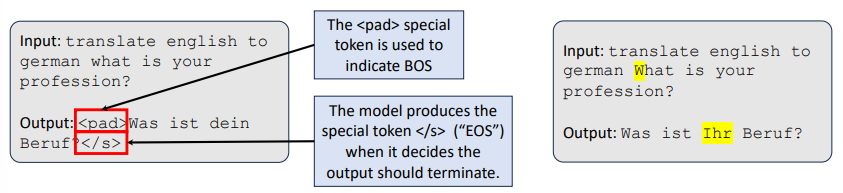
\includegraphics[width=0.3\linewidth]{content/Parts/images/2026-10-05-10-58-49.png}
\end{figure}

\begin{tcolorbox}
  \textbf{Note:} All model have their representation of EOF, in this case we have <\s>
\end{tcolorbox}


\subsection{Not instruction-tuned, yet!}
While it may resemble the behavior of instruction-tuned models (``chat-like
conversation''), that's not it!.
T5 is only tuned on specific tasks. The model learns to recognize those tasks and addresses them.

No strong generalization capabilities to new tasks


This means the model is not instruction-tuned! It is an initial model, but can solve multiple
things.

\begin{figure}[h!]
  \centering
  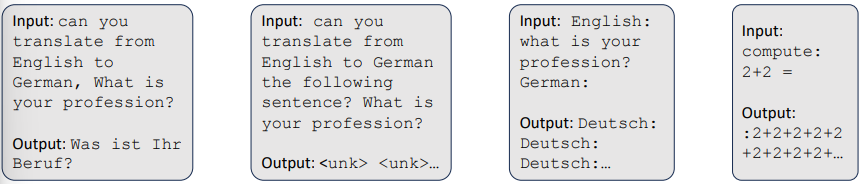
\includegraphics[width=0.3\linewidth]{content/Parts/images/2026-10-05-11-01-05.png}
\end{figure}


\section{Beyond encoder-decoder}


\subsection{Encoder-only architecture}



\begin{center}
  \begin{minipage}{0.65\linewidth}
    Encoder-only architectures primarily focus on
    understanding and encoding input data
    “without generating output”.


    The “decoder” part of the architecture is
    removed. The encoder is trained to solve some tasks.

    We have an input and want to do someting with this seuence e.g. classification, regression, name
    endity recognition, sentimental analysis, etc.
    and NOT want to generate a new sequence.



  \end{minipage}%
  \hfill
  \begin{minipage}{0.3\linewidth}
    \centering
    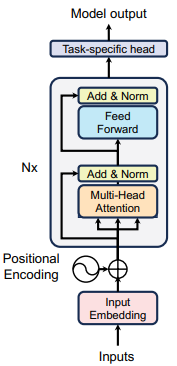
\includegraphics[width=0.3\linewidth]{content/Parts/images/2026-10-05-11-02-22.png}
  \end{minipage}
\end{center}


\subsection{BERT - Bidirectional Encoder Representations from Transformers}

This is arguably the most famous encoder-only transformer architecture.

It is pre-trained on two self-supervised tasks.

Pre-trained did the initial traingin on this task, but we can do the fine-tuning chanign a little
bit more the weights depends on out task. This process needs only few hundred sentences.


It uses bidirectional attention the endoer self-attention.

\begin{figure}[h!]
  \centering
  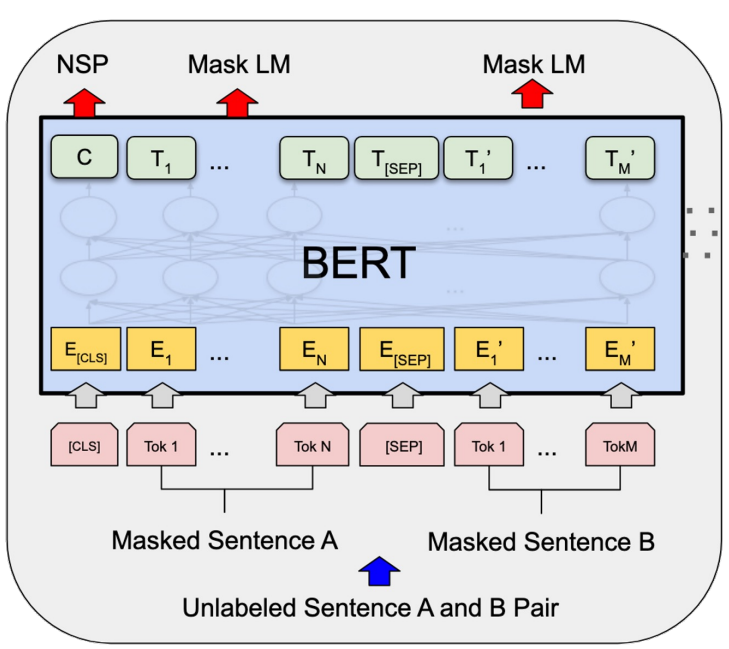
\includegraphics[width=0.3\linewidth]{content/Parts/images/2026-10-05-11-10-51.png}
\end{figure}

\subsection{Input encoding}


\begin{center}
  \begin{minipage}{0.65\linewidth}

    We have a token vector for each tocken, a positional embedding for each position and segment embedding with
    two vector  A and B used for question and answer.

    We intruduce the \textbf{segment embeddings}, they are two vectors, used by BERT allows to
    pass two sentences to the input of the model.
    This is usefull because traiinig is easyer and second one is allows the qeustion and answer


  \end{minipage}%
  \hfill
  \begin{minipage}{0.3\linewidth}
    \centering
    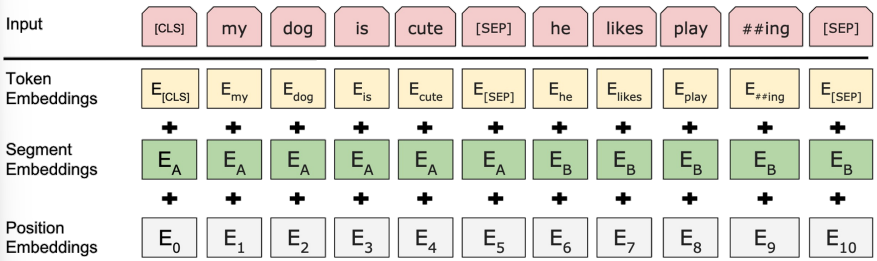
\includegraphics[width=0.3\linewidth]{content/Parts/images/2026-10-05-11-13-39.png}
  \end{minipage}
\end{center}

\subsection{Masked LM}

\begin{center}
  \begin{minipage}{0.65\linewidth}

    Google taken some sentences and removed some words, putting blanks. This is
    ~15\% of the words.
    The output of BERT is used to reconstruct the masked tockens.

    This classification task is called Masked LM. We predict the masked tokens using the linear and softmax
    activation functions.

  \end{minipage}%
  \hfill
  \begin{minipage}{0.3\linewidth}
    \centering
    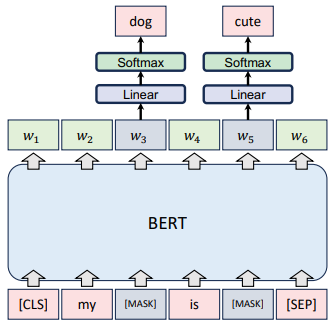
\includegraphics[width=0.3\linewidth]{content/Parts/images/2026-10-05-11-16-27.png}
  \end{minipage}
\end{center}

\subsection{Next Sentence Prediction}


\begin{center}
  \begin{minipage}{0.65\linewidth}

    This second task provides two sentences as input A and B. Is a self supervised task.

    We ask BERT if the sentence B have sense after sentence A. We train the model to havve understanding
    the consequntiality.

    Here one prediction for each sentence.

    We add an additonal tocken at the beginning of the sentence called CLS, and we use the output vector
    as the source the information.

    The limitation we cannot store of an entire paragraph in a vector, we need to compress,
    but this way is a good starting point.

  \end{minipage}%
  \hfill
  \begin{minipage}{0.3\linewidth}
    \centering
    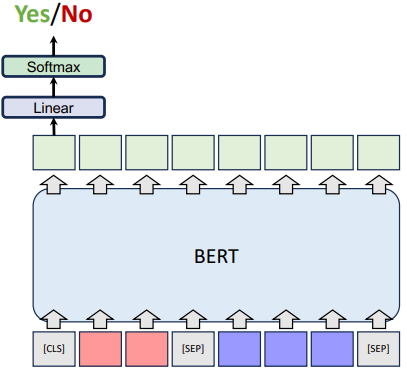
\includegraphics[width=0.3\linewidth]{content/Parts/images/2026-10-07-11-50-06.png}
  \end{minipage}
\end{center}


\subsection{Attention example in BERT}

Esample to encode a simple sentence: "[CLS] The dog ate the food because it was
hungry [SEP]".

BERT's attentions help understand how each
token is considered throughout the
transformer.

How many attention do we have?
BERT use 12 tranformers layers one after the other. Each layer has 12 heads meaning 12 application
of the attention mechanism.
The sentence ha 11 tokens. Eanch head produces $11 \times 11$ attention map.

For a total of 12 layers times 12 heads = 144 attention maps. Each map is a $11 \times 11$ matrix.


\begin{center}
  \begin{minipage}{0.65\linewidth}

    The attention bean paied to next token, and some time paid attention previous token.
    The vector weight is influenced by the dog word.


  \end{minipage}%
  \hfill
  \begin{minipage}{0.3\linewidth}
    \centering
    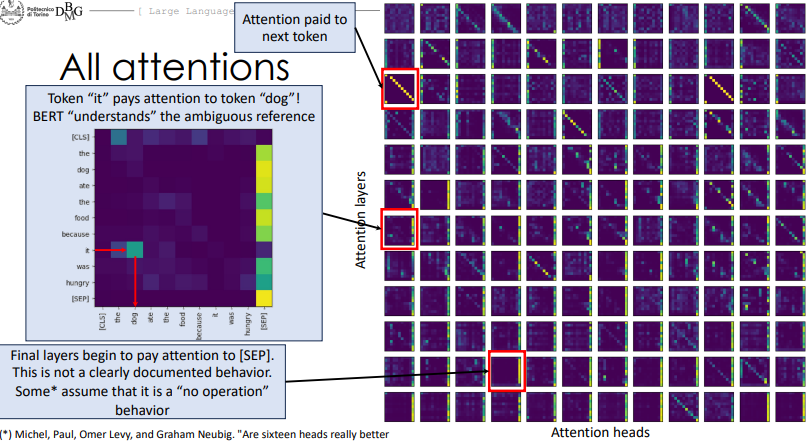
\includegraphics[width=0.3\linewidth]{content/Parts/images/2026-10-07-12-01-14.png}
  \end{minipage}
\end{center}


\subsection{Decoder-only architecture}

The most interesting part used today.

Is a type arch in witch we make a model extending a sequence. Just give the next token.
The rest of the output is generated in an \textbf{autoregressive} manner.

We do not have the encoder, the decoder already sees the input as the beginning of the output.

We dont ave the cross-attention, we use only the decoder self-attention. We use cross-attention
when we use multimodel model. GPT model family is a decoder-only architecture.

\subsection{GPT (Generative Pre-trainined Transformer)}




\begin{center}
  \begin{minipage}{0.65\linewidth}

    Decoder only transformer \textbf{pretrained} on the text generation task.
    Then, the model is \textbf{fine-tuned} on specific, supervised task.
    The model is provided the beginning of a sequence as the
    initial “decoder output”.

    \textbf{Greedy sampling} taks the most probable token at each step.

  \end{minipage}%
  \hfill
  \begin{minipage}{0.3\linewidth}
    \centering
    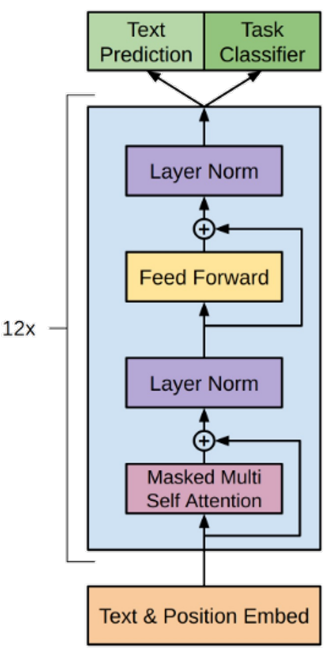
\includegraphics[width=0.3\linewidth]{content/Parts/images/2026-10-07-12-10-34.png}
  \end{minipage}
\end{center}


\section{Sampling approaches}

In order to chose the best token we need to use some teqniques. We have different stragegies usaully
used together.
In some cases, we want \textbf{deterministic} behaviors, in other cases we want \textbf{stochastic} behaviors.

\subsection{Some sampling approaches}

\begin{itemize}
  \item \textbf{Greedy sampling}: Select the token with the highest probability. It is deterministic. Bead beahavior when
        the model read repatitive sequences (repetition penalty)
  \item \textbf{Beam search}: Still deterministic. Keep some option and explore the most promising ones. We use \textit{k} how many
        parallel sentence adding the word
  \item \textbf{Random sampling}: Semantically has bit confuse
  \item \textbf{Top-k sampling}: I want to sample but not want long tails that has low prob. If high entropy
        very distributed.
  \item \textbf{Top-p sampling}: We want sample high prob. Instad of having a fixed k number of tokens, we select flexible
        k. The probability of the selected tokens is greater than p (95\% prob mass).
  \item \textbf{Temperature sampling}: lika random sampling changing the softmax. If T is 0 means greedy sampling (deterministic) case.
\end{itemize}























